\setchapterstyle{lines}
\chapter{Mean SPE Charge Distribution of DOMs}
\label{ch:spe_check}
One of the stages of the unblinding stage of the analysis presneted in \refch{HESE12} involved a strong Data-Monte Carlo disagreement between obsreved and expected number of Doubel Cascade events when DeepCore DOMs were included in the analysis. While DeepCore DOMs have been excluded from the previous iterations of this analysis \sidecite{Juliana_thesis,marcel_thesis} due to the bias they bring to \texttt{millipede} based reconstructions used in this analysis (see Section~\ref{sec:reco}), recent modifications in the simulations made it possible to use them again. Nevertheless, the access of observed double cascade events in 7.5 years of HESE data, initiated a series of detailed checks to understand the root of the problem, \emph{Why is inclusion of the  DeepCore DOMs causing a Data/Monte Carlo mismatch?}. The following section describes some issues observed in regards to single photoelctron (spe) charge templates used in simulation and data, that are used in \texttt{millipede} to calculate the observed light yield of the event. This work was done in collaboration with Jakob Van Santen\footnote{DESY - Deutsches Elektronen-Synchrotron
Platanenallee 6, D-15738, Zeuthen

email : jakob.van.santen@desy.de}.

In the Monte Carlo processing chain described in Section~\ref{sec:mc_sim}, at the Detetcor Simulation stage, the acceptance of a photon arriving at a Digital Optical Module (DOM) and the charge assigned to it are determined by several key factors. The acceptance is influenced by the global DOM efficiency, which scales the overall probability of photon detection, as well as the relative DOM efficiency, which accounts for variations in performance among individual DOMs. Additionally, angular acceptance curves are employed, which consider the interaction location and the angle of the photon relative to the DOM surface. This multi-faceted approach ensures a more accurate representation of the photon acceptance process\sidenote{Note that High QE DeepCore DOMs exhibit a distinctly different shape compared to  non-DeepCore DOMs, leading to a mean charge that is 3.6\% lower than that of NQE DOMs. To account for this difference, the compensation factor is adjusted to be 3.6\% higher (effectively resulting in a 3.6\% higher Relative DOM Efficiency, or RDE), ensuring that the total charge collected remains consistent following the implementation of the SPE Templates.}
To enhance the charge assignment, the new Single PhotoElectron (SPE) Templates (right panel of \reffig{SPE_oldnew}) have replaced the previous method (left panel of \reffig{SPE_oldnew}) of sampling from the general TA0003 charge distribution \sidecite{SPE_paper}. Each DOM now features a uniquely measured in-ice charge distribution, which is stored in the Geometry, Calibration, and Detector (GCD) file. This distribution is characterized by the sum of two exponential functions and a Gaussian, accurately reflecting the single-photoelectron response. Furthermore, the SPE Templates incorporate a global residual correction, a DOM efficiency scaling factor, and a charge scaling factor to account for shifts observed between processing passes. This comprehensive methodology enables the DOM Launcher to assign a charge that more accurately represents each DOM's behavior in the detector simulation.

\begin{figure*}[h!]
    \begin{subfigure}[h]{0.7\textwidth}
        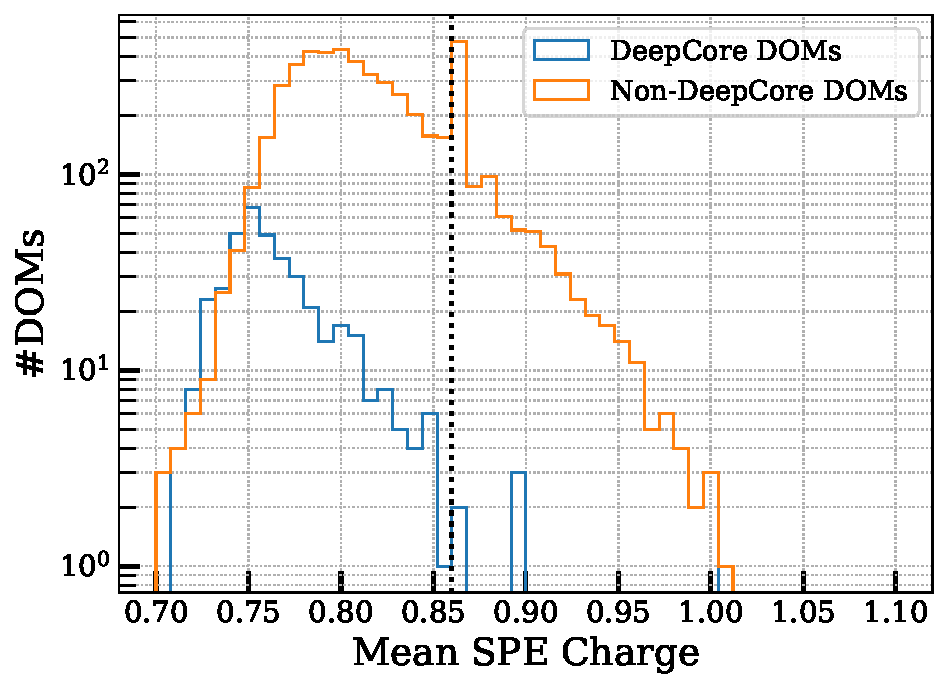
\includegraphics{./figures/results/Old.pdf}
    \end{subfigure}
    \hfill
    \begin{subfigure}[h]{0.7\textwidth}
        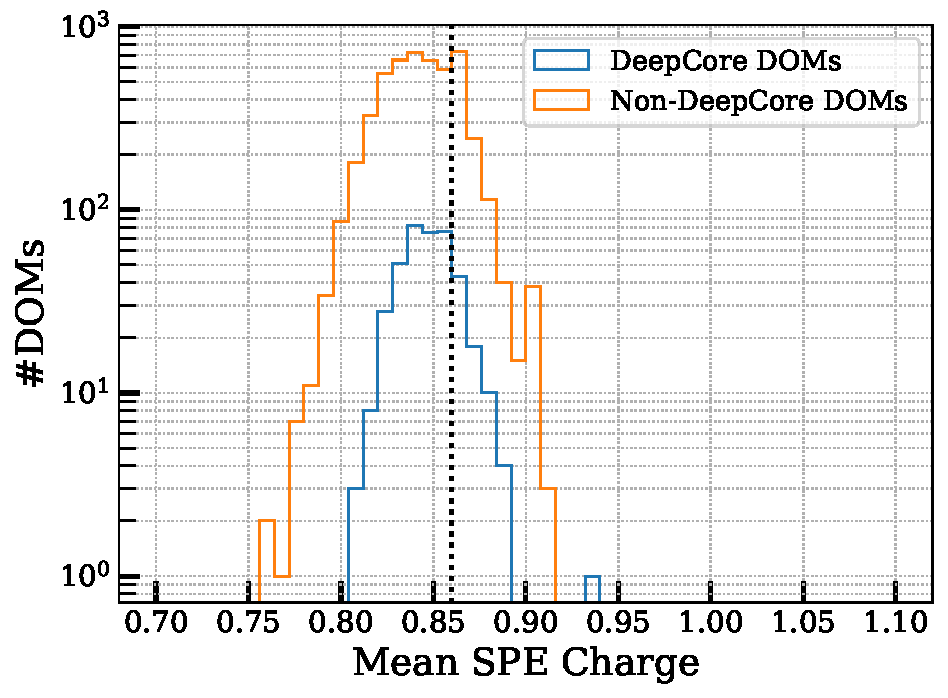
\includegraphics{./figures/results/simulation.pdf}
    \end{subfigure}
    
    \caption[Distribution of the Single Photoelectron (spe) charge for DOMs in data files]{Distribution of the Single Photoelectron (spe) charge for DOMs, shown separately for High Quantum Efficiency DeepCOre DOMs (blue) and for rest of the DOMs (orange). The vertical line shows the average SPE charge per DOM, after applying the compensation factor. Left Panel shows the old distribution, and right panel shows the updated distribution.}
    \labfig{SPE_oldnew}
\end{figure*}

While this update has been implemented in the simulation used for the analysis presented in this thesis, which employs the updated Single PhotoElectron (SPE) template (see \reffig{SPE_sim}), the corresponding data files were not updated with this new parameterization until 2023. The Data GCD files still contained the parameterization based on the old template, as illustrated in the left panel of \reffig{SPE_oldnew}. The figures show the distribution of mean SPE charge for both DeepCore and Non-DeepCore DOMs. Notably, the old template reveals a significantly larger deviation (greater than 10\%) for DeepCore DOMs compared to Non-DeepCore DOMs, which display only about a 5\% deviation. This occurs against a backdrop where the mean SPE charge is approximately 0.85, where we define 1 PE as the mean of the Gaussian component of the SPE charge distribution. It’s important to note that while this value represents 1 PE, the distribution is not purely Gaussian and includes a population below the valley, leading to an average value of less than 1.
\begin{marginfigure}
    
    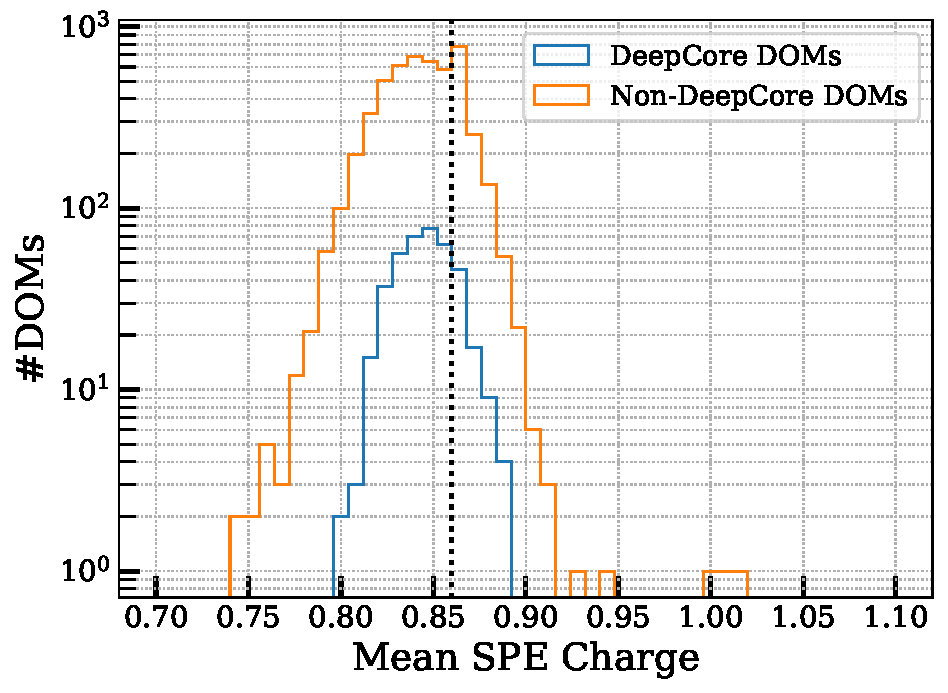
\includegraphics{./figures/results/Updated.pdf}


    \caption[Distribution of the Single Photoelectron (spe) charge for DOMs in simulation]{Distribution of the Single Photoelectron (spe) charge distribution for DOMs used in Simulation. See caption of \reffig{SPE_oldnew} for details.}
    \labfig{SPE_sim}
\end{marginfigure}
The lack of observation of this effect in previous iterations of the analysis can likely be attributed to the fact that these variations are primarily observed in DeepCore DOMs, which were initially excluded from the analysis. The 5\% difference observed among Non-DeepCore DOMs can be effectively compensated for by the DOM Efficiency nuisance parameter, denoted as \(\eta_{\mathrm{domeff}}\), which is incorporated in the fit and allowed to vary within 10\% of its nominal range. While it remains inconclusive whether the excess of observed double cascades was due to the inaccurate parameterization of the SPE template, it is evident that updating all existing GCD files for the data would be necessary to substantiate this claim, a task that lies beyond the scope of this thesis work. The study ultimately concludes that, for the sake of achieving better Data-Monte Carlo agreement, a straightforward solution would be to remove the DeepCore DOMs from the reconstruction process. This approach simplifies the comparison between the SPE template distributions available for the Data (left panel of \reffig{SPE_oldnew}) and the one utilized in the simulation (see \reffig{SPE_sim}).






\setchapterstyle{lines}
\chapter{Validity Of Wilks' Theorem}
\label{ch:wilks}
Throughout this thesis, the results (\refch{HESE12}) and sensitivity analyses (\refch{analysis}) have been presented under the assumption that Wilks' theorem is valid. Wilks' theorem is a statistical approximation that simplifies the interpretation of likelihood ratios by predicting that the log-likelihood ratio will follow a \(\chi^2\)-distribution with \(k\) degrees of freedom \sidecite{Wilks_thm}. It is given as,



\begin{equation}\label{eq:ts_distribution}
TS = -2ln\frac{\mathcal{L}_{\text{fixed}}}{\mathcal{L}_{\text{free}}} = -2 \ln \left( \frac{\mathcal{L} \left( n \,|\, \mu \left( f_{\nu_e} = \hat{\hat{f}}_{\nu_e}^{\text{s.p.}}, \, f_{\nu_\tau} = \hat{\hat{f}}_{\nu_\tau}^{\text{s.p.}}, \, \theta, \, \xi \right) \right)}{\mathcal{L} \left( n \,|\, \mu \left( f_{\nu_e}, \, f_{\nu_\tau}, \, \theta, \, \xi \right) \right)} \right)
\end{equation}
where, \(\hat{\hat{f}}_{\nu_e}^{\text{s.p.}}\) and \(\hat{\hat{f}}_{\nu_\tau}^{\text{s.p.}}\): Conditional best-fit values for electron and tau neutrino flavor compositions, where flavor fractions are fixed at specific values during the scan. \(\hat{f}_{\nu_e}\) and \(\hat{f}_{\nu_\tau}\): Values of flavor compositions for free fits, where parameters can vary freely. \(\theta\): Remaining model parameters, such as astrophysical normalization and the spectral index. \(\xi\): Nuisance parameters accounting for uncertainties not directly of interest.

Here, \(k\) is defined as the difference in degrees of freedom between the tested model (with likelihood \(\mathcal{L}_{\text{fixed}}\)) and the model that best fits the data (with likelihood \(\mathcal{L}_{\text{free}}\)). This approximation, however, relies on several conditions for accuracy: (1) the tested hypothesis must be a nested case of the free-fit hypothesis, meaning the tested model is a subset of the parameters of the best-fit model, (2) neither the parameters of interest nor nuisance parameters can be bounded (they must be able to vary freely to any values), and (3) the sample size \(n\) must be large to ensure the distribution converges to \(\chi^2\).

The first condition of nested hypotheses is satisfied. For example, when testing for different astrophysical flavor compositions or constraining the tau neutrino contribution, the tested models serve as special cases of the unconstrained model, having fewer degrees of freedom. However, the remaining two conditions are more problematic. The flavor fractions, for instance, are constrained to positive values, meaning that the parameters of interest are restricted to never go below zero. While not all of the nuisance parameters are not exactly restricted by a bound, the atmospheric spectra norms are also restricted to be positive, always. This violates the second assumption. Lastly, the HESE sample size is relatively small (with only a handful of double cascades from tau neutrinos and a total of < 200 events). While this doesn't necessarily mean that wilks' theorem does not hold anymore, an assessment is required to verify its validity.


\begin{figure}[h!]
    
    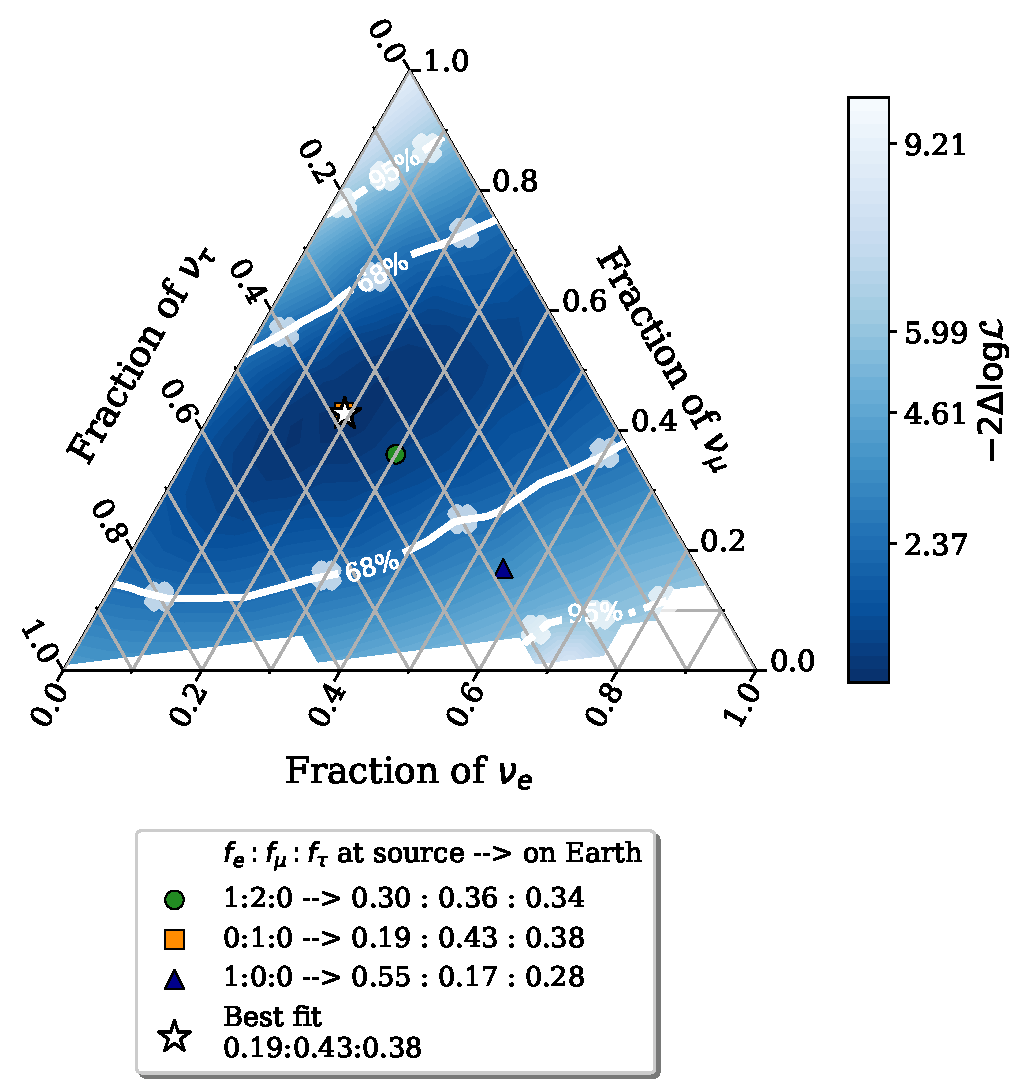
\includegraphics{./figures/results/HESE12_fancy_coverage.pdf}


    \caption[Illustration of the selected scan points to check coverage in phase space of astrophysical neutrino flavour fractions]{Illustration of the selected scan points to check coverage in phase space of astrophysical neutrino flavour fractions. The profile likelihood scan is same as in \reffig{flavour_comp}, representing 68\% (solid) and 95\% (dashed) confidence region.}
    \labfig{trial_coverage}
\end{figure}

This is done by comparing the coverage of the test statistic distribution from the monte carlo pseudo experiments to the coverage of $\chi_{k=2}^2$. The coverage was tested at various points along the 68\% and 95\% confidence contours to check if the log-likelihood ratio truly followed the expected \(\chi^2\)-distribution. Five representative points were selected along each confidence contour (see \reffig{trial_coverage}), and 500\sidenote{The nubers of trials was selected to keep statistical errors low for the points on 68\%, as for 95\%, the numbers of trials need to be as high as 1000, which becomes computationally expensive. Idea was to check for any significant deviations on 68\% region and later produce more trials if needed for points on 95\% contours.} pseudo datasets were generated at each of these points by injecting a specific flavor composition (indicated by 'x' on the plot) while holding the other model parameters at their best-fit values given in \reftab{bf_nuisance} and \reftab{bf_signal}. Each pseudo dataset was fitted twice: once with the flavor composition fixed to the injected point, and once allowing all parameters to vary freely. A likelihood ratio test was applied to each trial by taking the ratio of the likelihoods from the free and fixed fits.

\begin{figure}[h!]
    
    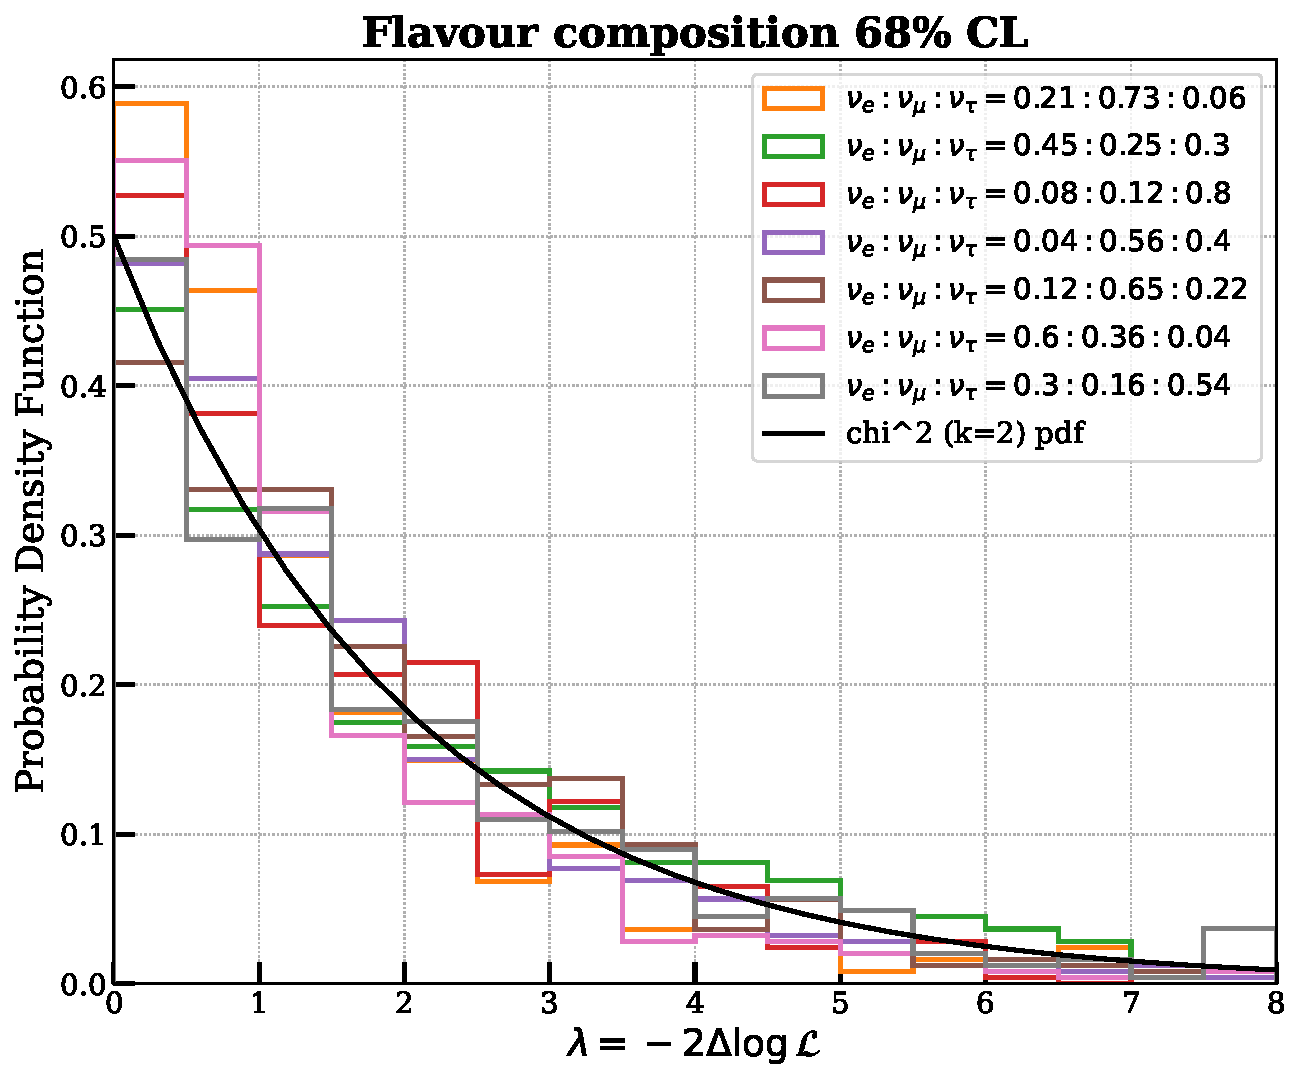
\includegraphics{./figures/results/wilkscheck_68CL.pdf}


    \caption[The TS distributions for each scan point at the 68\% confidence levels (shown in \reffig{trial_coverage})]{The TS distributions for each scan point at the 68\% confidence levels (shown in \reffig{trial_coverage}). The likelihood ratio is defined in Equation~\ref{eq:ts_distribution}. Each distribution results from injecting the corresponding flavor compositions (indicated also in the plot legend) into the Monte Carlo simulation, as described in the text. Statistical uncertainties are omitted for clarity. A $\chi^2$-distribution with two degrees of freedom is included for comparison in each plot.}
    \labfig{68_wilks}
\end{figure}

\begin{figure}[h!]
    
    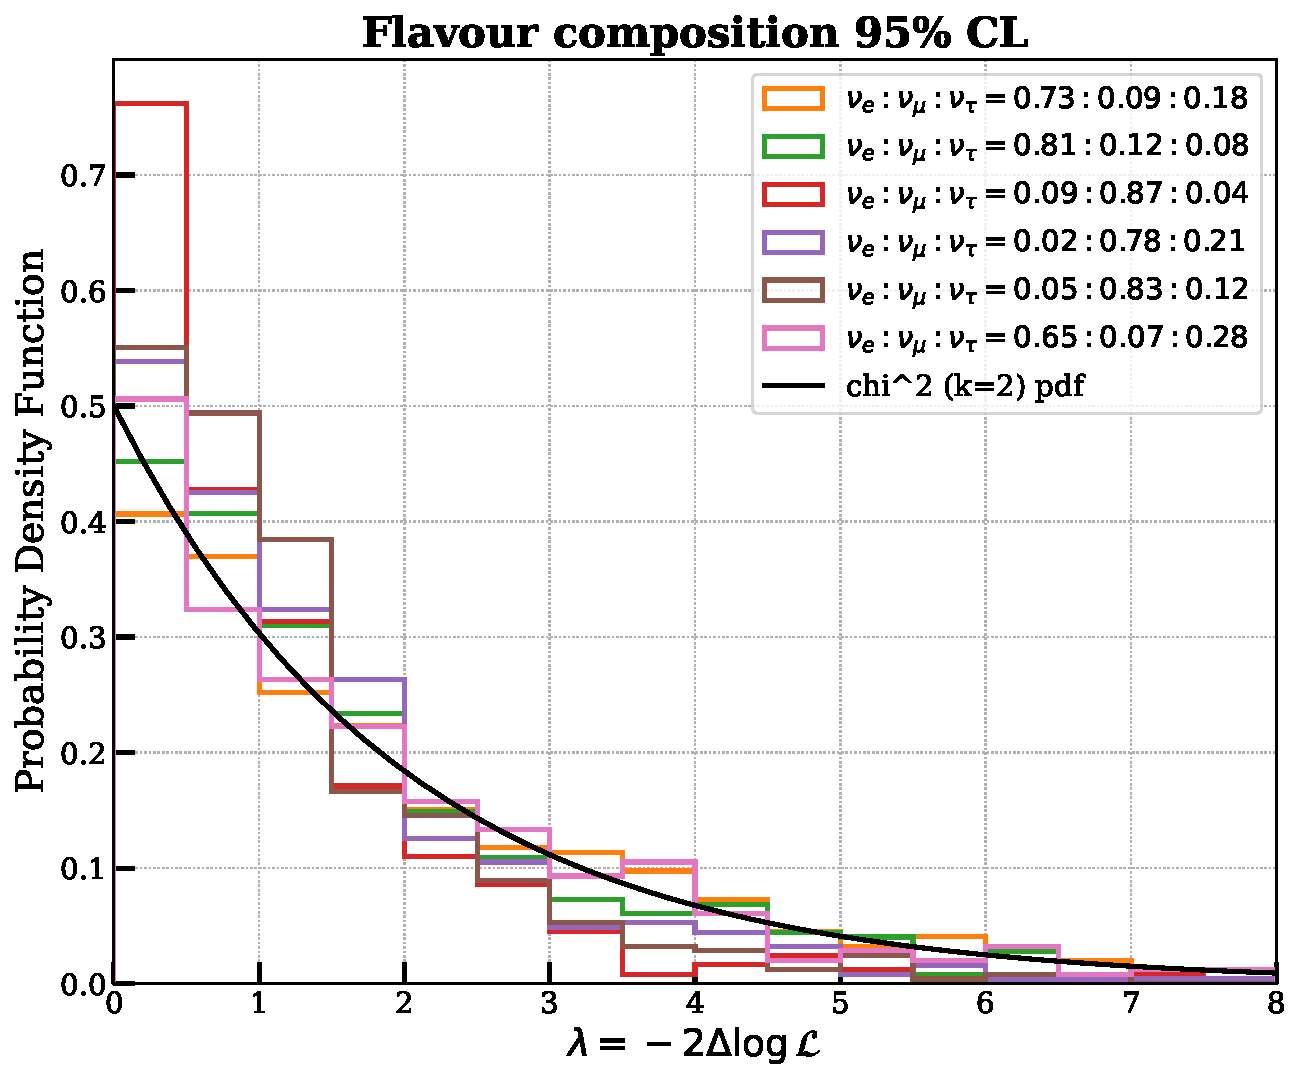
\includegraphics{./figures/results/wilkscheck_95CL.pdf}


    \caption[The TS distributions for each scan point at the 95\% confidence levels]{The TS distributions for each scan point at the 95\% confidence levels. See caption of \reffig{68_wilks} for details.}
    \labfig{95_wilks}
\end{figure}

The distribution of the test statistic (TS), represented by \(-2 \Delta \log \mathcal{L}\), was then compared to a \(\chi^2\)-distribution with \(k=2\) degrees of freedom (shown as a black line) to assess if it conformed to the expected distribution. \reffig{68_wilks} shows the TS distributions for points along the 68\% confidence contour, and \reffig{95_wilks} shows the distributions for points along the 95\% contour. Although minor deviations were observed in some of the TS distributions, these deviations were not significant enough to indicate a substantial departure from Wilks' theorem. An exact fit to the \(\chi^2\)-distribution is not fully expected, as there is some correlation between the two fitting parameters, likely reducing the effective degrees of freedom to just below 2. In addition, some of the points (especially the ones on 95\% contour) are in a phase space of the triangle whice often fit experiences minimisation faliure due to large deviation from the best-fit values. Overall, Wilks' theorem appears to hold consistently across the entire parameter space, indicating that it should also be valid for the true physical parameter values. Therefore, Wilks' theorem can be reliably used for both one- and two-dimensional parameter scans, enabling the calculation of confidence intervals presented in Section~\ref{sec:flavour_results} for deriving the main results and in Section~\ref{sec:sensitivty} for determining the sensitivity.


\setchapterstyle{lines}
\chapter{Sensitivity Estimation using Monte Carlo PseudoTrials}
\label{ch:sensitivity_checks}
The sensitivty derived at best-fit using an asimov dataset \sidecite{asimov} was discussed in \ref{sec:sens_bf}. In \reffig{PEs}, the marroon line shows asimov sensitivity of the analysis at the best-fit, which predicts that ideally, analysis should be able to put tighter constraints on the measured flavour fraction (specifically the $\nu_tau$ fraction). As there is a strong mismatch between results and the sensitivty, a test was made to generate sensitivity estimation using monte carlo pseudo trials.

Construction of monte carlo pseudo datasets and TS distribution is done in the similar way as it was done in Appendix~\ref{ch:wilks} with two main differences. First, instead of a few points on the contours, a grid across entire triangle is considered (see blue + in \reffig{trial_points}), each of which (about 500) represents the points for which a pseudo dataset were generated. Second, unlike the case of coverage test, in this case, conditional best-fit, i.e \(\hat{\hat{f}}_{\nu_e}^{\text{s.p.}}\) and \(\hat{\hat{f}}_{\nu_\tau}^{\text{s.p.}}\) in \ref{eq:ts_distribution} is \textbf{always} kept at signal bestfit values of flavour fractions ($f_{\nu_e} = 0.19$ and $f_{\nu_{tau}}=0.38$), for every set of trials. The goal of this approach is to capture the potential variability in the TS under different hypothetical "true" parameter configurations and to understand how likely the best-fit hypothesis would be rejected if any of these points were the actual parameter values. By spanning the parameter space, we also avoid any bias toward the best-fit configuration, providing a fair estimate of sensitivity.

A critical first step is the selection of injected points within the parameter space of the flavour triangle. \reffig{trial_points} shows the grid of injected points chosen to span the entire range of flavour compositions, extending beyond the best-fit values, $\nu_e:\nu_{\mu}:\nu_{\tau} = 0.19:0.43:0.38$. This approach ensures a comprehensive sensitivity estimate across various possible configurations. For each of these injected points, a corresponding pseudo dataset was generated to simulate observations that would arise if the true parameter values were equal to the injected values.

\begin{figure}[h]
    
    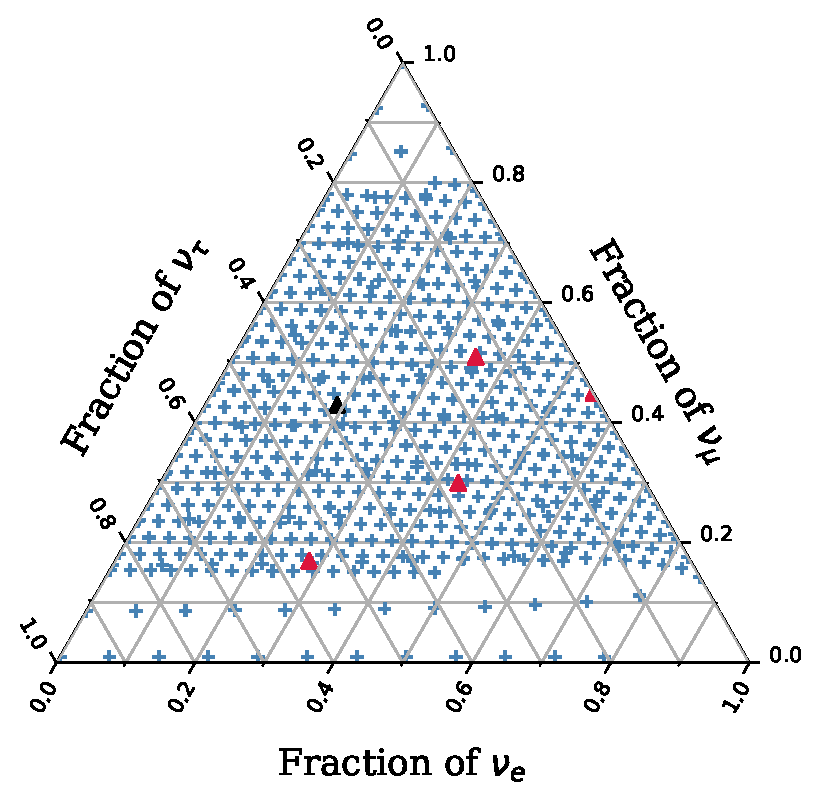
\includegraphics{./figures/results/trials_points.pdf}


    \caption[Illustartion of various points on the flavour composition phase space, used in sensitivity derivation]{Illustartion of various points on the flavour composition phase space, used in sensitivity derivation. Each + represents a pseudo dataset, drawn from flavour composition of that very point. The best-fit flavour composition of $\nu_e:\nu_{\mu}:\nu_{\tau} = 0.19:0.43:0.38$ is indicated with a black triangle, while the few TS distributions discussed in \reffig{TS_ofrandom} and text are shown with red triangle. All other parameters of the fit are injected at their bestfit values.}
    \labfig{trial_points}
\end{figure}

\begin{figure}[h!]
    
    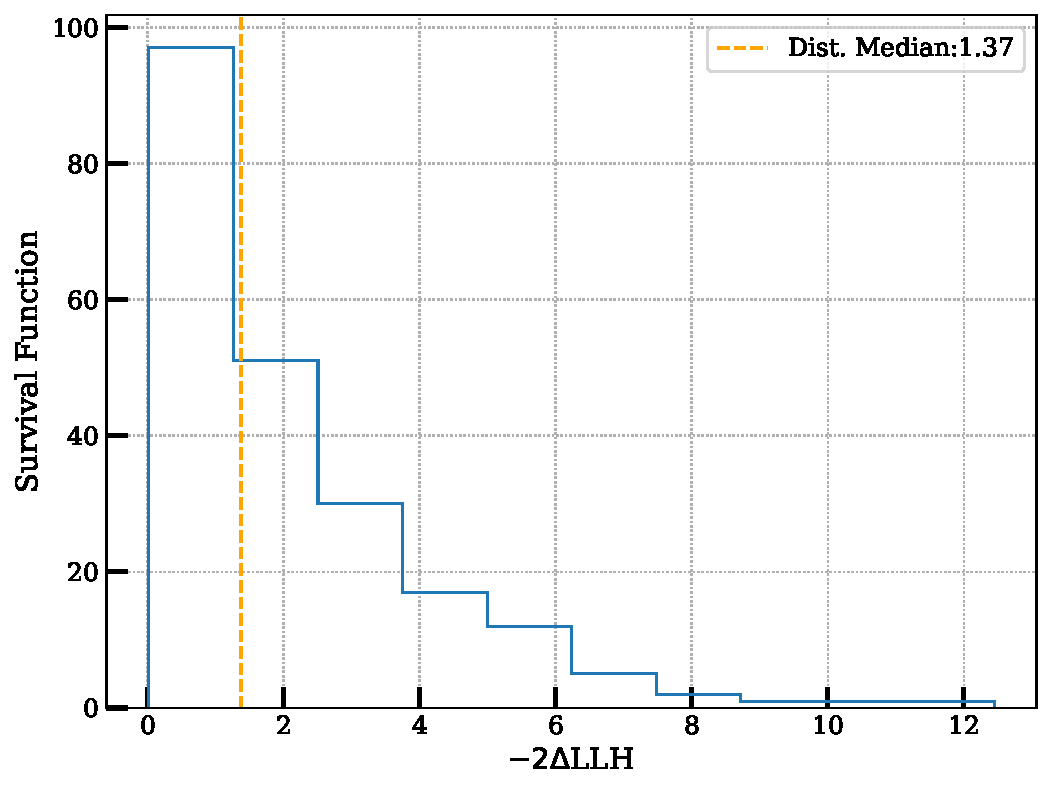
\includegraphics{./figures/results/median_atbestfit_TS.pdf}


    \caption[The distribution of TS of pseudo dataset produced by injecting best-fit flavour composition (black triangle in \reffig{trial_points})]{The distribution of TS of pseudo dataset produced by injecting best-fit flavour composition (black triangle in \reffig{trial_points}). TS is calculated using likelihood ratio defined in \ref{eq:ts_distribution}}, by taking ratio of conditional best-fit (flavour fractions fixed at best-fit values) to free fit. The vertical line shows median of the distribution that serves as a critical TS for the rest of the trial' TS distributions.
    \labfig{TS_bestfit}
\end{figure}
To interpret the TS values derived from each pseudo dataset, a critical value needs to be established first. For this purpose, a TS distribution is generated using, pseudo data generated at best-fit values and fitted twice in the same manner described before. This distribution is displayed in \reffig{TS_bestfit}, which shows the TS survival function under the best-fit hypothesis with the median value marked. This median TS value serves as a critical threshold, allowing us to evaluate the TS values obtained from pseudo datasets generated at other injected points. If a pseudo dataset generated at an alternative parameter configuration produces a TS greater than the critical TS, the dataset provides evidence against the best-fit hypothesis at the corresponding confidence level, in other words, the fraction of pseudo datasets injected at a given points below the critical value gives significance with which best-fit hypothesis can be rejected. 

\begin{figure*}[hbt!]

\begin{subfigure}{.7\textwidth}
    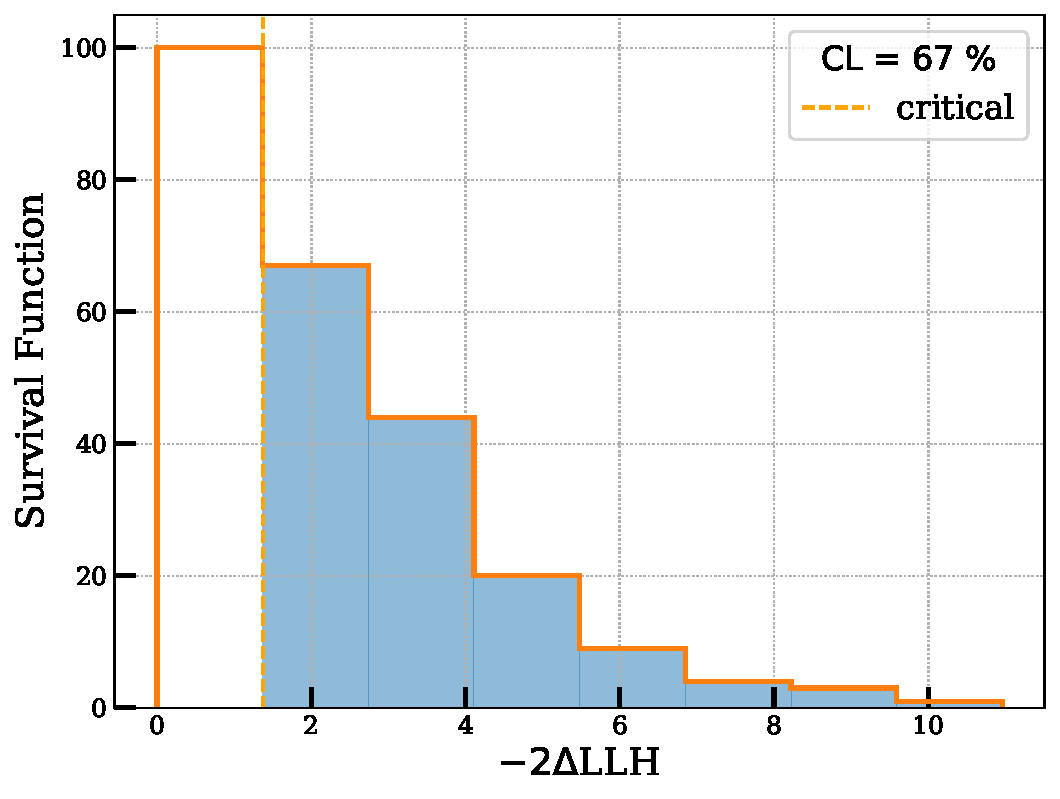
\includegraphics[width=\linewidth]{./figures/results/67_distribution.pdf}
    \caption{injected point $\nu_e:\nu_{\mu}:\nu_{\tau} = 0.35:0.51:0.14$}
    \labfig{67_TS}
\end{subfigure}\hfill % <-- "\hfill"
\begin{subfigure}{.7\textwidth}
    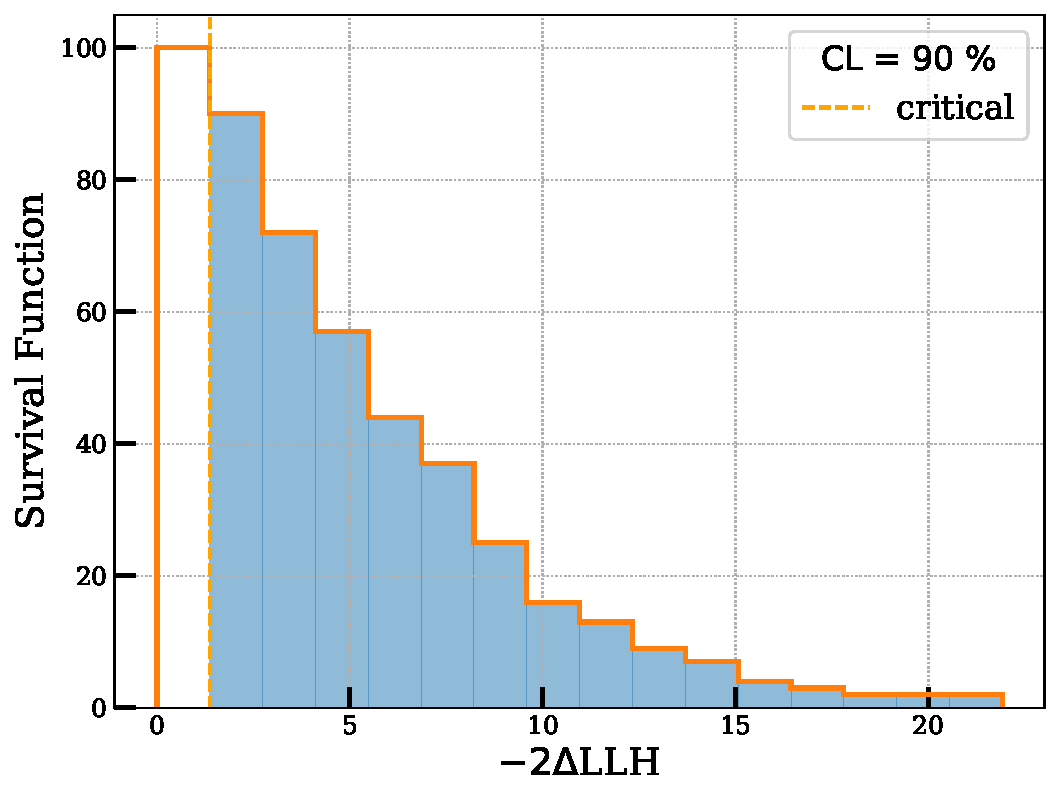
\includegraphics[width=\linewidth]{./figures/results/90_distribution.pdf}
    \caption{injected point $\nu_e:\nu_{\mu}:\nu_{\tau} = 0.55:0.445:0.0$}
    \labfig{90_TS}
\end{subfigure}

\medskip % create some *vertical* separation between the graphs
\begin{subfigure}{.7\textwidth}
    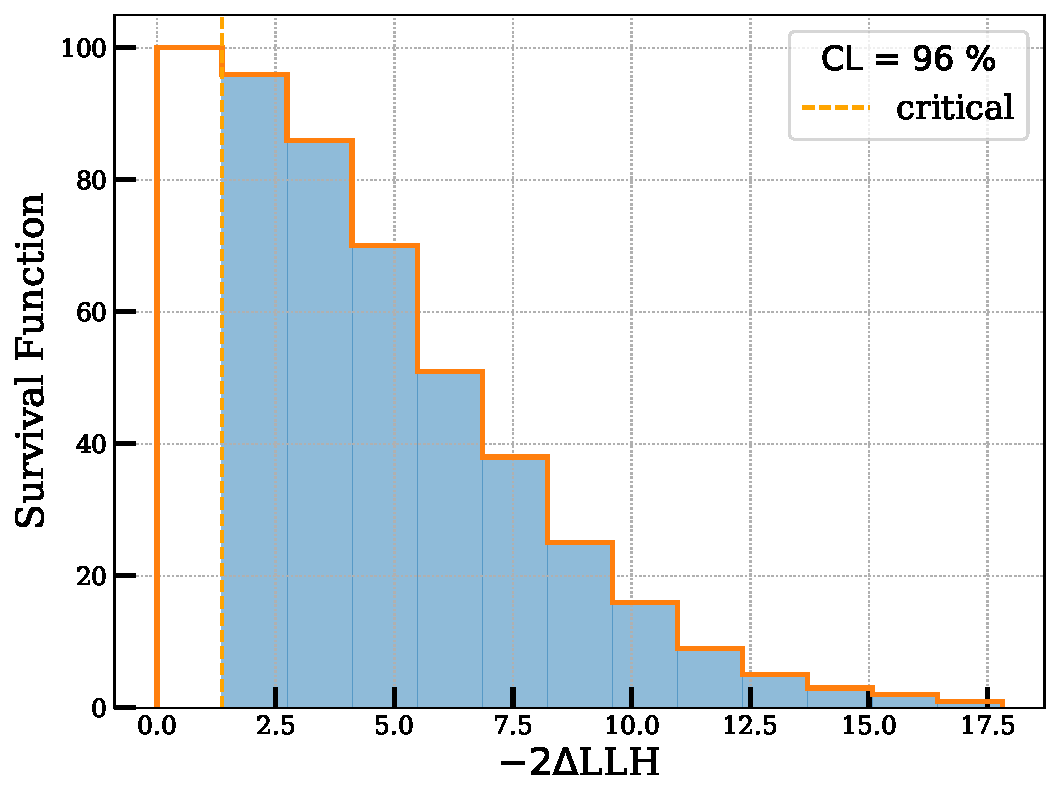
\includegraphics[width=\linewidth]{./figures/results/96_distribution.pdf}
    \caption{injected point $\nu_e:\nu_{\mu}:\nu_{\tau} = 0.43:0.3:0.27$}
    \labfig{96_TS}
\end{subfigure}\hfill % <-- "\hfill"
\begin{subfigure}{.7\textwidth}
    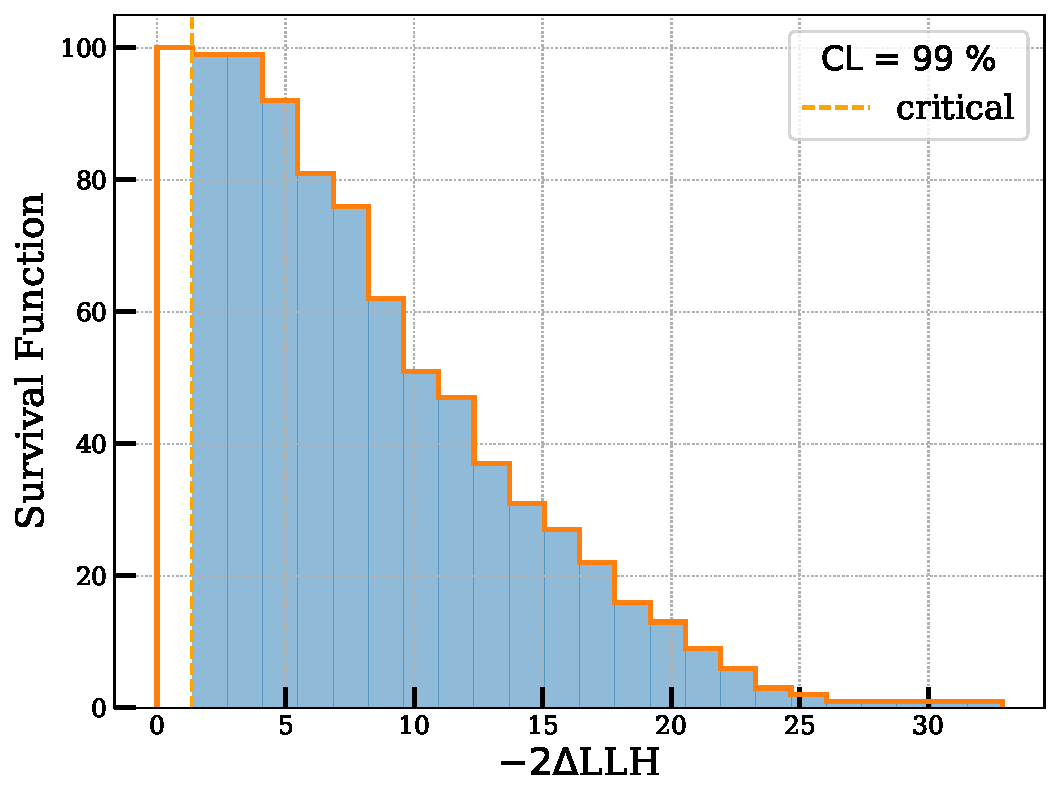
\includegraphics[width=\linewidth]{./figures/results/99_distribution.pdf}
    \caption{injected point $\nu_e:\nu_{\mu}:\nu_{\tau} = 0.28:0.17:0.55$}
    \labfig{99_TS}
\end{subfigure}

\caption[The distribution of TS for pseudo datasets generated by injecting various best-fit flavor compositions (indicated below each plot and by red triangles in \reffig{trial_points})]{The distribution of TS for pseudo datasets generated by injecting various best-fit flavor compositions (indicated below each plot and by red triangles in \reffig{trial_points}) is shown. The shaded regions represent the fraction of trials exceeding the critical value defined in \reffig{TS_bestfit}. This fraction, indicated on each plot, conveys the confidence level (CL) with which the best-fit hypothesis is rejected.}
\labfig{TS_ofrandom}
\end{figure*}


\reffig{TS_ofrandom} displays the survival distributions of TS values for four specific injected points (indicated with red triangle in \reffig{trial_points}), each corresponding to different confidence levels (67\%, 90\%, 96\%, and 99\%). In each figure, the fraction of the TS distribution that exceeds the median TS benchmark for the best-fit hypothesis is highlighted as a shaded orange region. These shaded areas represent the fraction of pseudo datasets, generated for each injected configuration, that yield a TS value above this critical threshold. This fraction quantifies the probability that the analysis would reject the best-fit hypothesis if the true values of flavour fractions correspond to the injected values used for each pseudo dataset. Therefore, these survival distributions illustrate how distinguishable each injected configuration is from the best-fit hypothesis, providing a clear measure of the sensitivity of the analysis.

After calculating the TS distributions for each injected point and comparing them to the critical threshold, we aggregate the results across all injected points to construct confidence intervals. \reffig{PEs} displays these sensitivity-derived confidence intervals, representing the regions in parameter space where the analysis is sensitive enough to distinguish between the best-fit hypothesis and alternative configurations at specified confidence levels (e.g., 90\% or 95\%). 

The implications of the results are discussed in detail in Section~\ref{sec:flavour_results}, but the point to take away is asimov sensitivity derived at the best-fit is rather stricter and analysis is in-fact sensitive to measure the flavour ratio (especially the $\nu_{\tau}$ fraction) of astrophysical neutrinos. 






